% Adjusting chapter title format for regular (numbered) chapters
\titleformat{\chapter}[display]
  {\normalfont\huge\bfseries\centering}{\chaptertitlename\ \thechapter}{20pt}{\Huge}

% Using similar styling for unnumbered chapters but without "Chapter" prefix
\titleformat{name=\chapter,numberless}
  {\normalfont\huge\bfseries\centering}{}{0pt}{\Huge}

\titlespacing*{\chapter}{0pt}{50pt}{40pt} % Adjust vertical spacing before and after the title

\chapter{Proposed Framework} % Ensures chapter numbering starts correctly
\label{chp:3}

\section{Proposed Approach}

\begin{figure*}[h]
  \centering
  \begin{tikzpicture}[component/.style={fill=gray!80, text=white,
      rounded corners, outer sep=1mm, text width=2.6cm, align=flush
      center, minimum height=1.2cm, scale=0.8},
    input/.style={draw, scale=0.8,  inner sep=2mm, outer sep=1mm}]\sf
    
    \foreach \x/\al/\lab in {%
      1/sampl/Sampling,%
      2/gener/Testcase Generation,%
      3/testing/Validation,%
      4/summary/{Error\\ Summarisation}%
    }{ \node[component] (\al) at (3.5*\x,0) {\textbf{\lab}}; }

    \node[fit=(sampl)(summary), draw=gray, ultra thick] (approach) {};

    \node[input] (aisystem) at (0.2, 0.5) {AI System $\S$};
    \node[input] (spec)     at (0.2, -0.5) {Specifications $\Sigma$};

    \foreach/\from/\to in {%
      sampl/gener, gener/testing, testing/summary%
    }{ \draw[-stealth, very thick] (\from) -- (\to); }

    \draw[-latex, thick] (aisystem) -- (approach.179);
    \draw[-latex, thick] (spec) -- (approach.181);
  \end{tikzpicture}
  \caption{Overview of the Proposed Framework}
  \label{fig:framework}
\end{figure*}

This section introduces our comprehensive approach to evaluating AI system performance, summarized in Figure~\ref{fig:framework}. It takes as input the description of an AI system and a set of relevant specifications against which the AI system should be checked. The framework itself has four main components:

\begin{enumerate}[\it (i)]
    \item \emph{Sampling}: Choosing the original inputs for the AI system.
    \item \emph{Testcase Generation}: Generating specific test cases from the sampled inputs according to the specifications.
    \item \emph{Validation}: Checking the behavior of the AI system on the generated test cases, which can be fully-fledged \emph{verification} or more lightweight \emph{testing}.
    \item \emph{Error Summarization}: Quantifying the performance of the AI system in terms of its global/local robustness/correctness.
\end{enumerate}

We focus on AI systems with DNN components performing classification tasks. We assume that an AI system $\S$ is a pair $(\F,\D)$ where:
\begin{itemize}
    \item $\F$ is the functional unit consisting of $n$ DNN \emph{classifiers} $f_1,\dots,f_n$ and a symbolic (software) component~$\omega$ such that given an input $\avec{x}=(x_1,\dots,x_n)$, the \emph{output}~$\F(\avec{x})$ is defined as $\omega(f_1(x_1),\dots,f_n(x_n))$.
    \item $\D$ (for dataset) is a structure that describes valid inputs for each classifier $f_i$ and the corresponding correct outputs (i.e., labels). In particular, $\D.\mathit{next}_i(\mathit{param})$ returns a valid input $x_i$ for $f_i$, given the parameter $\mathit{param}$. Moreover, $\D.N_i$ is the number of distinct class labels for each classifier~$f_i$.
\end{itemize}

\begin{example}
\label{ex:mnist-adder}
An instance of a simple AI system is an \emph{MNIST Digit Adder} $\S_{\text{MNIST}} = (\F,\D)$, where $\F = (\{f_{\text{mnist}}\}, +)$, $f_{\text{mnist}}$ is an MNIST Digit classifier and $\F$ takes as input two MNIST Digit images, recognizes the digits in the images, and computes their sum, i.e., $\F(x_1,x_2) = f_{\text{mnist}}(x_1) + f_{\text{mnist}}(x_2)$. $\D$ is the testing dataset for MNIST Digit consisting of 10,000 labeled images.
\end{example}

We assume that \emph{specifications} $\Sigma$ is a pair $(P, V)$, where $P$ is a set of perturbations against which we are characterizing the behavior of $\S$. Each perturbation comes with parameters to instantiate the set of all possible perturbations. $V$ is a validation flag, where if $V=t$, then we do testing, and if $V=v$, we do verification.

\begin{example}
To evaluate the correctness of the MNIST Digit Adder $\S_{\text{MNIST}}$, we define the specifications $\Sigma = (P, V)$ as follows: $P = \{\gaussian(0,0.1), \saltpepper(200:255, 0:5, 0.2), \rotation(3,30,3)\}$ and $V=t$. Here, $\gaussian(0,0.1)$ specifies Gaussian noise with a mean of $0$ and standard deviation of $0.1$, $\saltpepper(200:255,0:5,0.2)$ specifies salt and pepper noise, where 10\% of pixels are bleached up to values 200 to 255 and 10\% of pixels are darkened to values between 0 and 5, and $\rotation(3,30,3)$ specifies the set of rotations with the minimum rotation angle of 3, maximum of 30, and the step size of 3.
\end{example}

\section{Sampling}

The sampling process involves a random but balanced choice of samples from each class, focusing exclusively on instances that the model has correctly predicted. Sampling happens independently for each classifier $f_i$. To ensure a representative and fair distribution of data across all classes, we sample the same number of instances from each class. The full sample $S_i$ for classifier $f_i$, $i=1,\dots,n$, is computed as:

\begin{equation}
S_i = \bigcup_{c=1}^{\D.N_i} S_i^c
\end{equation}

where $S_i^c$ is a subset of the correctly classified samples for a class $c$ consisting of $M_i$ (the number of samples for each class specific to $f_i$) elements:
\[S_i^c = \big\{x = \D.next_i(class=c)\mid f_i(x)=c\big\}|_{M_i}\] 
Note that each sample is obtained by a call to the method $\D.next_i$.

\begin{example}
Recall the MNIST Digit Adder system $\S_{\text{MNIST}}$ from Example~\ref{ex:mnist-adder}. When sampling, we make sure to select only correctly classified samples. For each digit $c$ (0 to 9), we randomly sample 100 images, i.e., $samp_1(\D,c,100)$ contains 100 inputs $x$ such that $f_{\text{mnist}}(x) = c$. In total, $S_1$ contains 1000 samples for all 10 classes.
\end{example}

\section{Test Case Generation}

The test case generation process aims to create test cases based on the given specifications to evaluate the correctness/robustness of the AI system.

Let $S_i^c$ be the set of samples produced in the sampling step for the classifier $f_i$ and a class $c$. For each perturbation $p\in P$, we generate a set $\T_p^c$ of test cases. Specifically, for each sample $x\in S$ we produce $testcases(p,c,x)$ according to $p$. Then $\T_p^c = \bigcup_{x\in S} testcases(p,c,x)$.

\begin{example}
To generate test cases for the MNIST Digit Adder $\S_{\text{MNIST}}$, we use the specifications defined in Example 2, which include noise and rotation perturbations. Let $S$ be the set of sampled images obtained in Example 3. For each pair of images $(x_1, x_2) \in S$, we define the following test cases:
\begin{itemize}
    \item \textbf{Rotation}: For a given angle $\theta$, generate the perturbed images $x_1' = \text{rotate}(x_1, \theta)$ and $x_2' = \text{rotate}(x_2, \theta)$. The test case is then:
    $\mathcal{T}_{\text{rotation}} = \left\{(x_1', x_2') \mid x_1', x_2' \in \text{rotate}(S, \theta)\right\}$
    \item \textbf{Noise}: For a given mean $\mu$ and standard deviation $\sigma$, generate the perturbed images $x_1'' = \text{noise}(x_1, \mu, \sigma)$ and $x_2'' = \text{noise}(x_2, \mu, \sigma)$. The test case is then:
    $\mathcal{T}_{\text{noise}} = \left\{(x_1'', x_2'') \mid x_1'', x_2'' \in \text{noise}(S, \mu, \sigma)\right\}$
\end{itemize}
The overall set of test cases $\mathcal{T}$ is the union of the individual test cases:
$\mathcal{T} = \mathcal{T}_{\text{rotation}} \cup \mathcal{T}_{\text{noise}}$
\end{example}

\section{Validation}

In this step, we run the validation queries for each test case generated previously. Let $f_i$ be a classifier, $x$ an input, and $c$ the correct class label of $x$. Denote by $query(f_i,x,c)$ the outcome of the validation query defined as $1$ if $f_i(x)=c$ and as $0$ otherwise. 

Fix $p\in P$ and a class $c$. For every test case in $\T_p^c$, we store the results in the form:
\[Raw_{p,c} = \Big\{\big(query(f_i,x,c),\ f_i(x)_c\big) \mid x \in \T_p^c\Big\}\]

After generating test cases, measure the AI subsystem's confidence for each class under each type of property.

\subsubsection{Local Correctness}

Local correctness involves checking the AI subsystem's performance on individual images subjected to different transformations. For each image $x$ from a set of samples $X$, the AI subsystem produces a confidence score $f(x)$ representing its certainty in recognizing the digit. The local correctness for a transformation $T$ applied to an image $x$ is defined as:

\[ \text{Local Correctness}(x, T) = f(T(x)) \]

where $T$ can be any transformation such as noise addition, rotation, brightness adjustment, occlusion, or scaling. Each transformation is evaluated to determine its impact on the confidence score.

\subsubsection{Global Correctness}

Global correctness evaluates the AI subsystem's performance on combinations of images and transformations, such as adding two digits under different transformations. Given a set of 100 samples for each digit (0-9), we randomly select images to form digit pairs. The global correctness assesses the combined confidence for recognizing the result of operations like addition under each transformation.

For each transformation $T$, we define local correctness for digits $d_1$ and $d_2$ as follows:

\[ \text{LC}_{T}(d_1) = \text{Local Correctness}(x_1, T) \]
\[ \text{LC}_{T}(d_2) = \text{Local Correctness}(x_2, T) \]

where $x_1$ and $x_2$ are randomly selected images representing digits $d_1$ and $d_2$.

The global correctness for each transformation is then defined as the product of the local correctness values:

\[ \text{GC}_{T} = \text{LC}_{T}(d_1) \times \text{LC}_{T}(d_2) \]

To determine the optimistic and pessimistic global correctness across all transformations, we calculate the following:

\begin{itemize}
    \item \textbf{Optimistic Global Correctness}:
    \[ \text{GC}_{opt} = \max_{T} (\text{GC}_{T}) \]
    \item \textbf{Pessimistic Global Correctness}:
    \[ \text{GC}_{pes} = \min_{T} (\text{GC}_{T}) \]
\end{itemize}

For the addition operation, if we denote the sum of digits $d_1$ and $d_2$ as $d_{\text{sum}}$, the overall global correctness for the operation is:

\[ \text{Overall Global Correctness} = \min(\text{GC}_{opt}, \text{GC}_{pes}) \]

where each transformation is evaluated separately, and the global correctness is determined based on the individual probabilities of correct recognition for each digit under each transformation.

\begin{figure}[h]
    \centering
    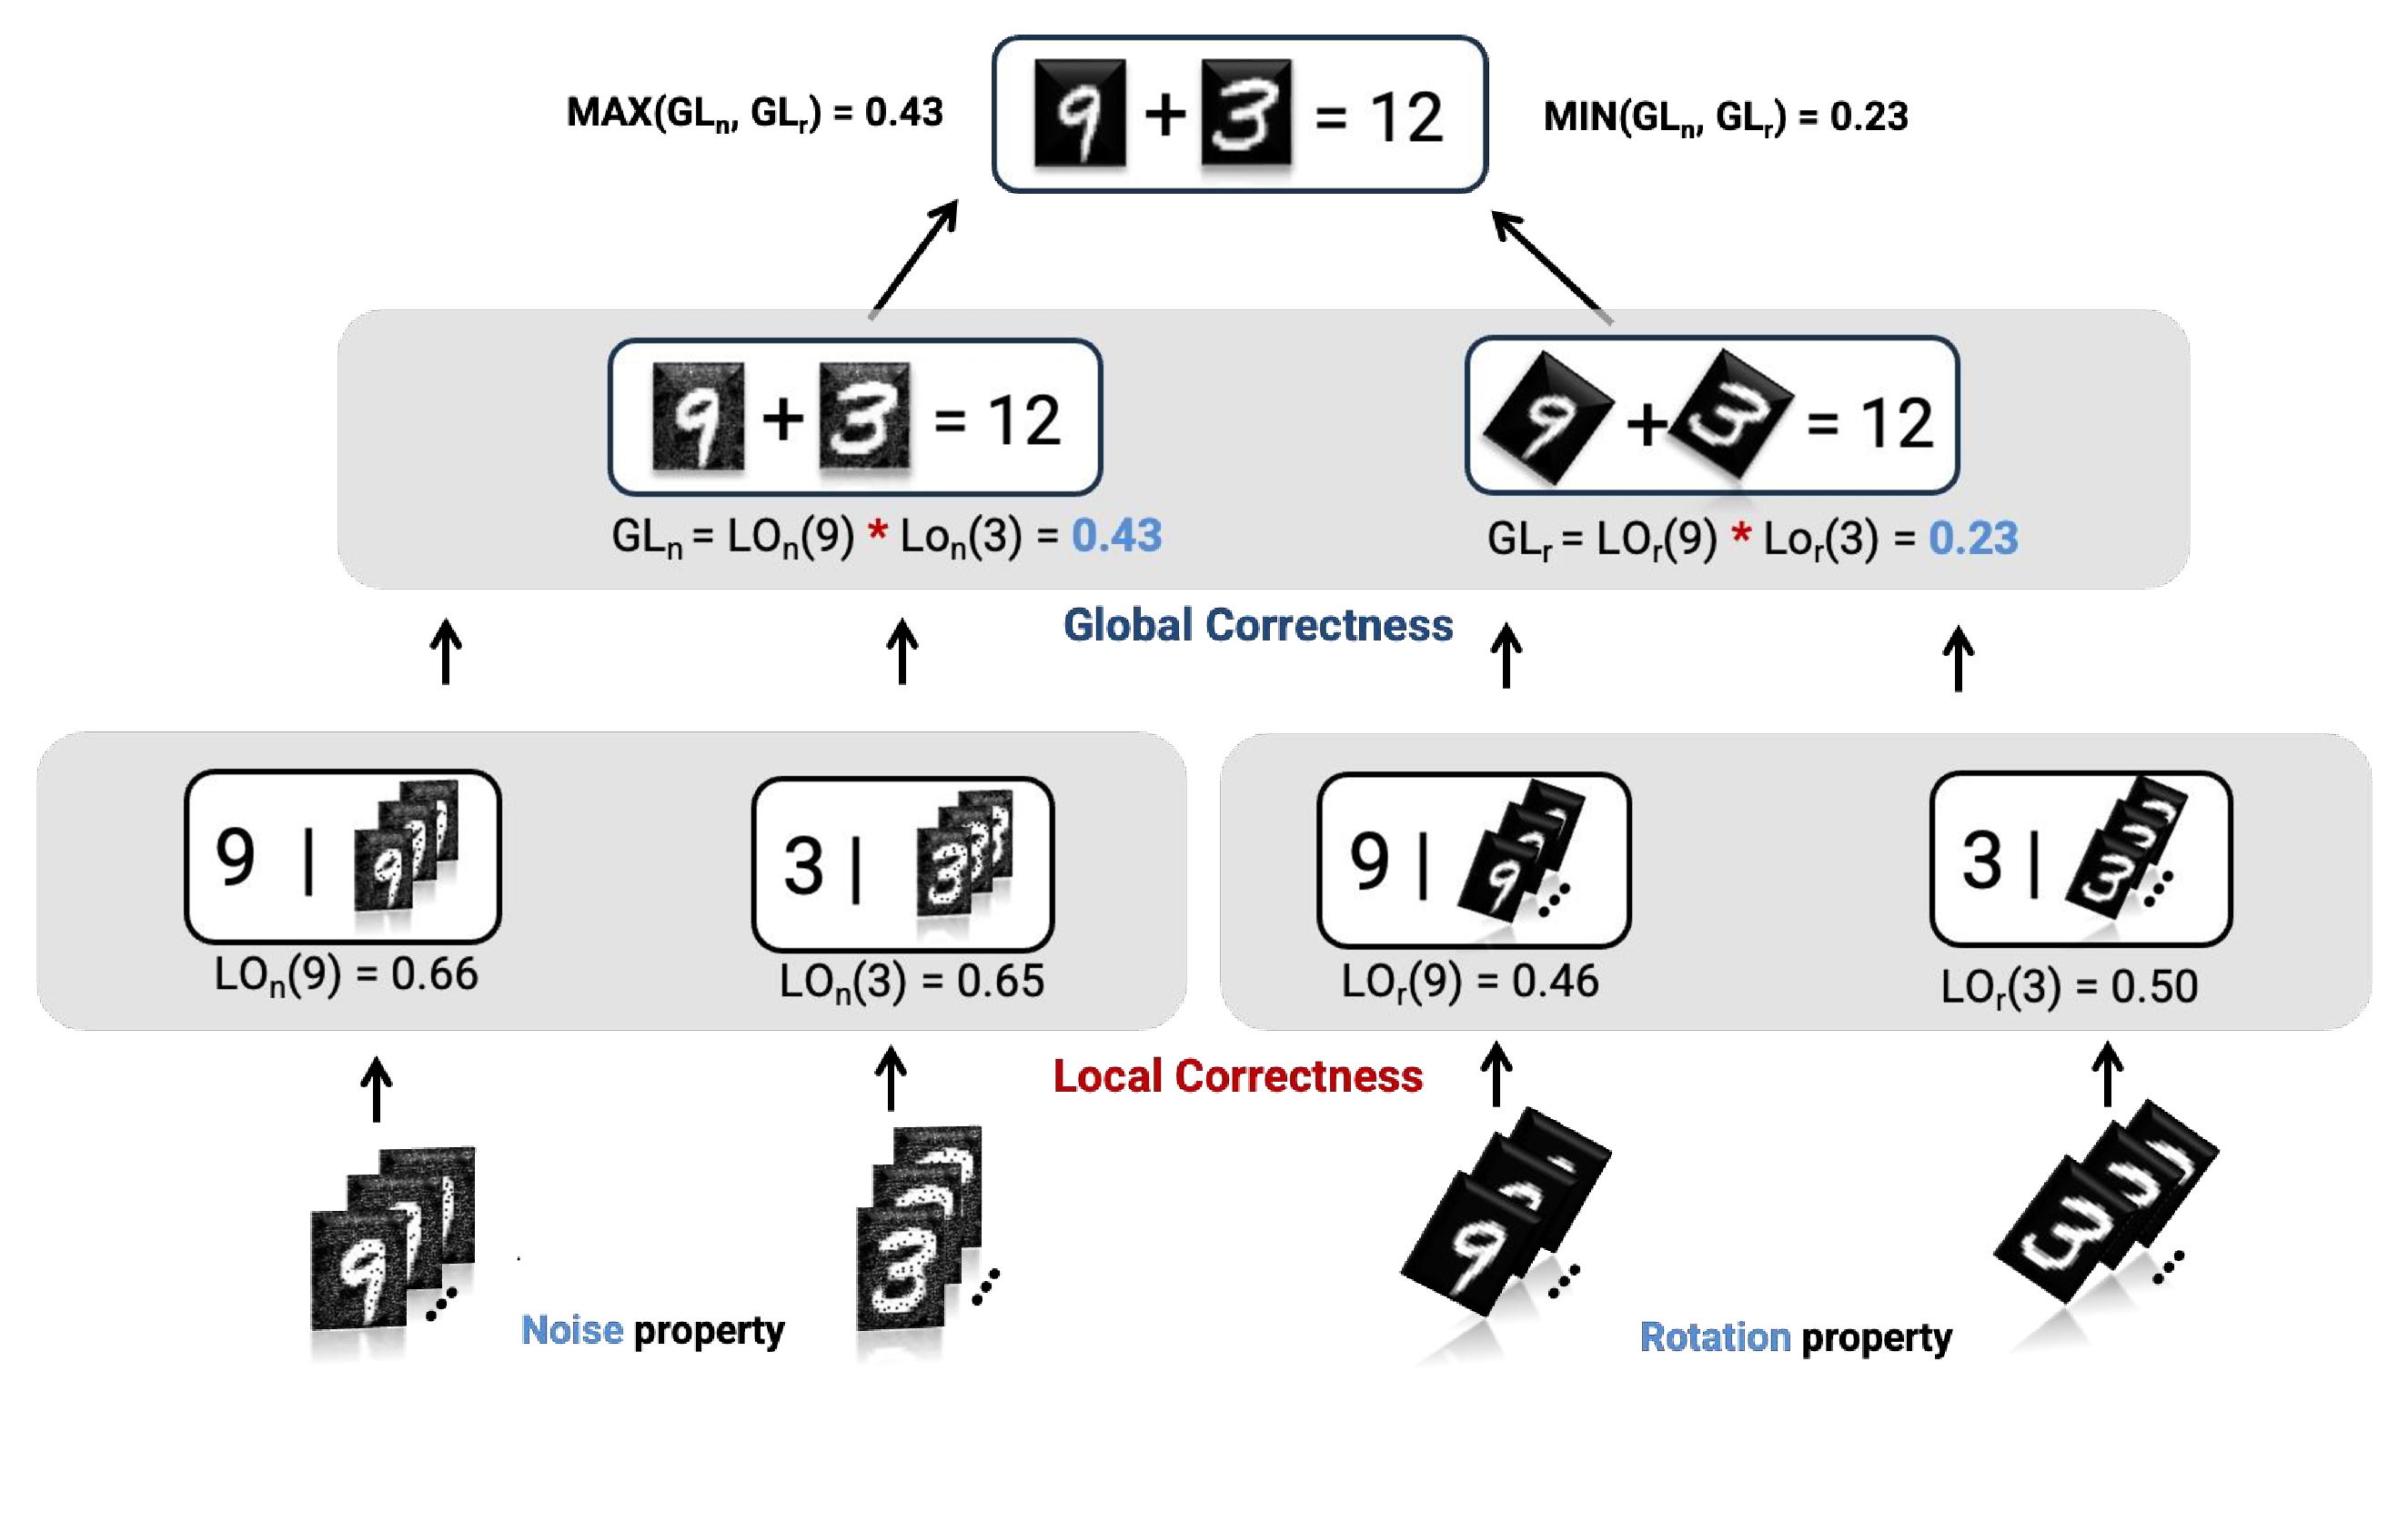
\includegraphics[width=\linewidth]{figures/noise_rotation_localcal_global.pdf}
    \caption{Graphical View of Local and Global Correctness}
    \label{fig:graph}
\end{figure}

\section{Error Summarization}

Error summarization involves evaluating the performance of the AI system by identifying and quantifying errors. We use Bayesian Network-based Coverage Metrics to assess both local and global coverage. Two testing coverage metrics are defined in Figure~\ref{Coverage}: local coverage (LC) and global coverage (GC).

\begin{figure*}[h]
    \centering
    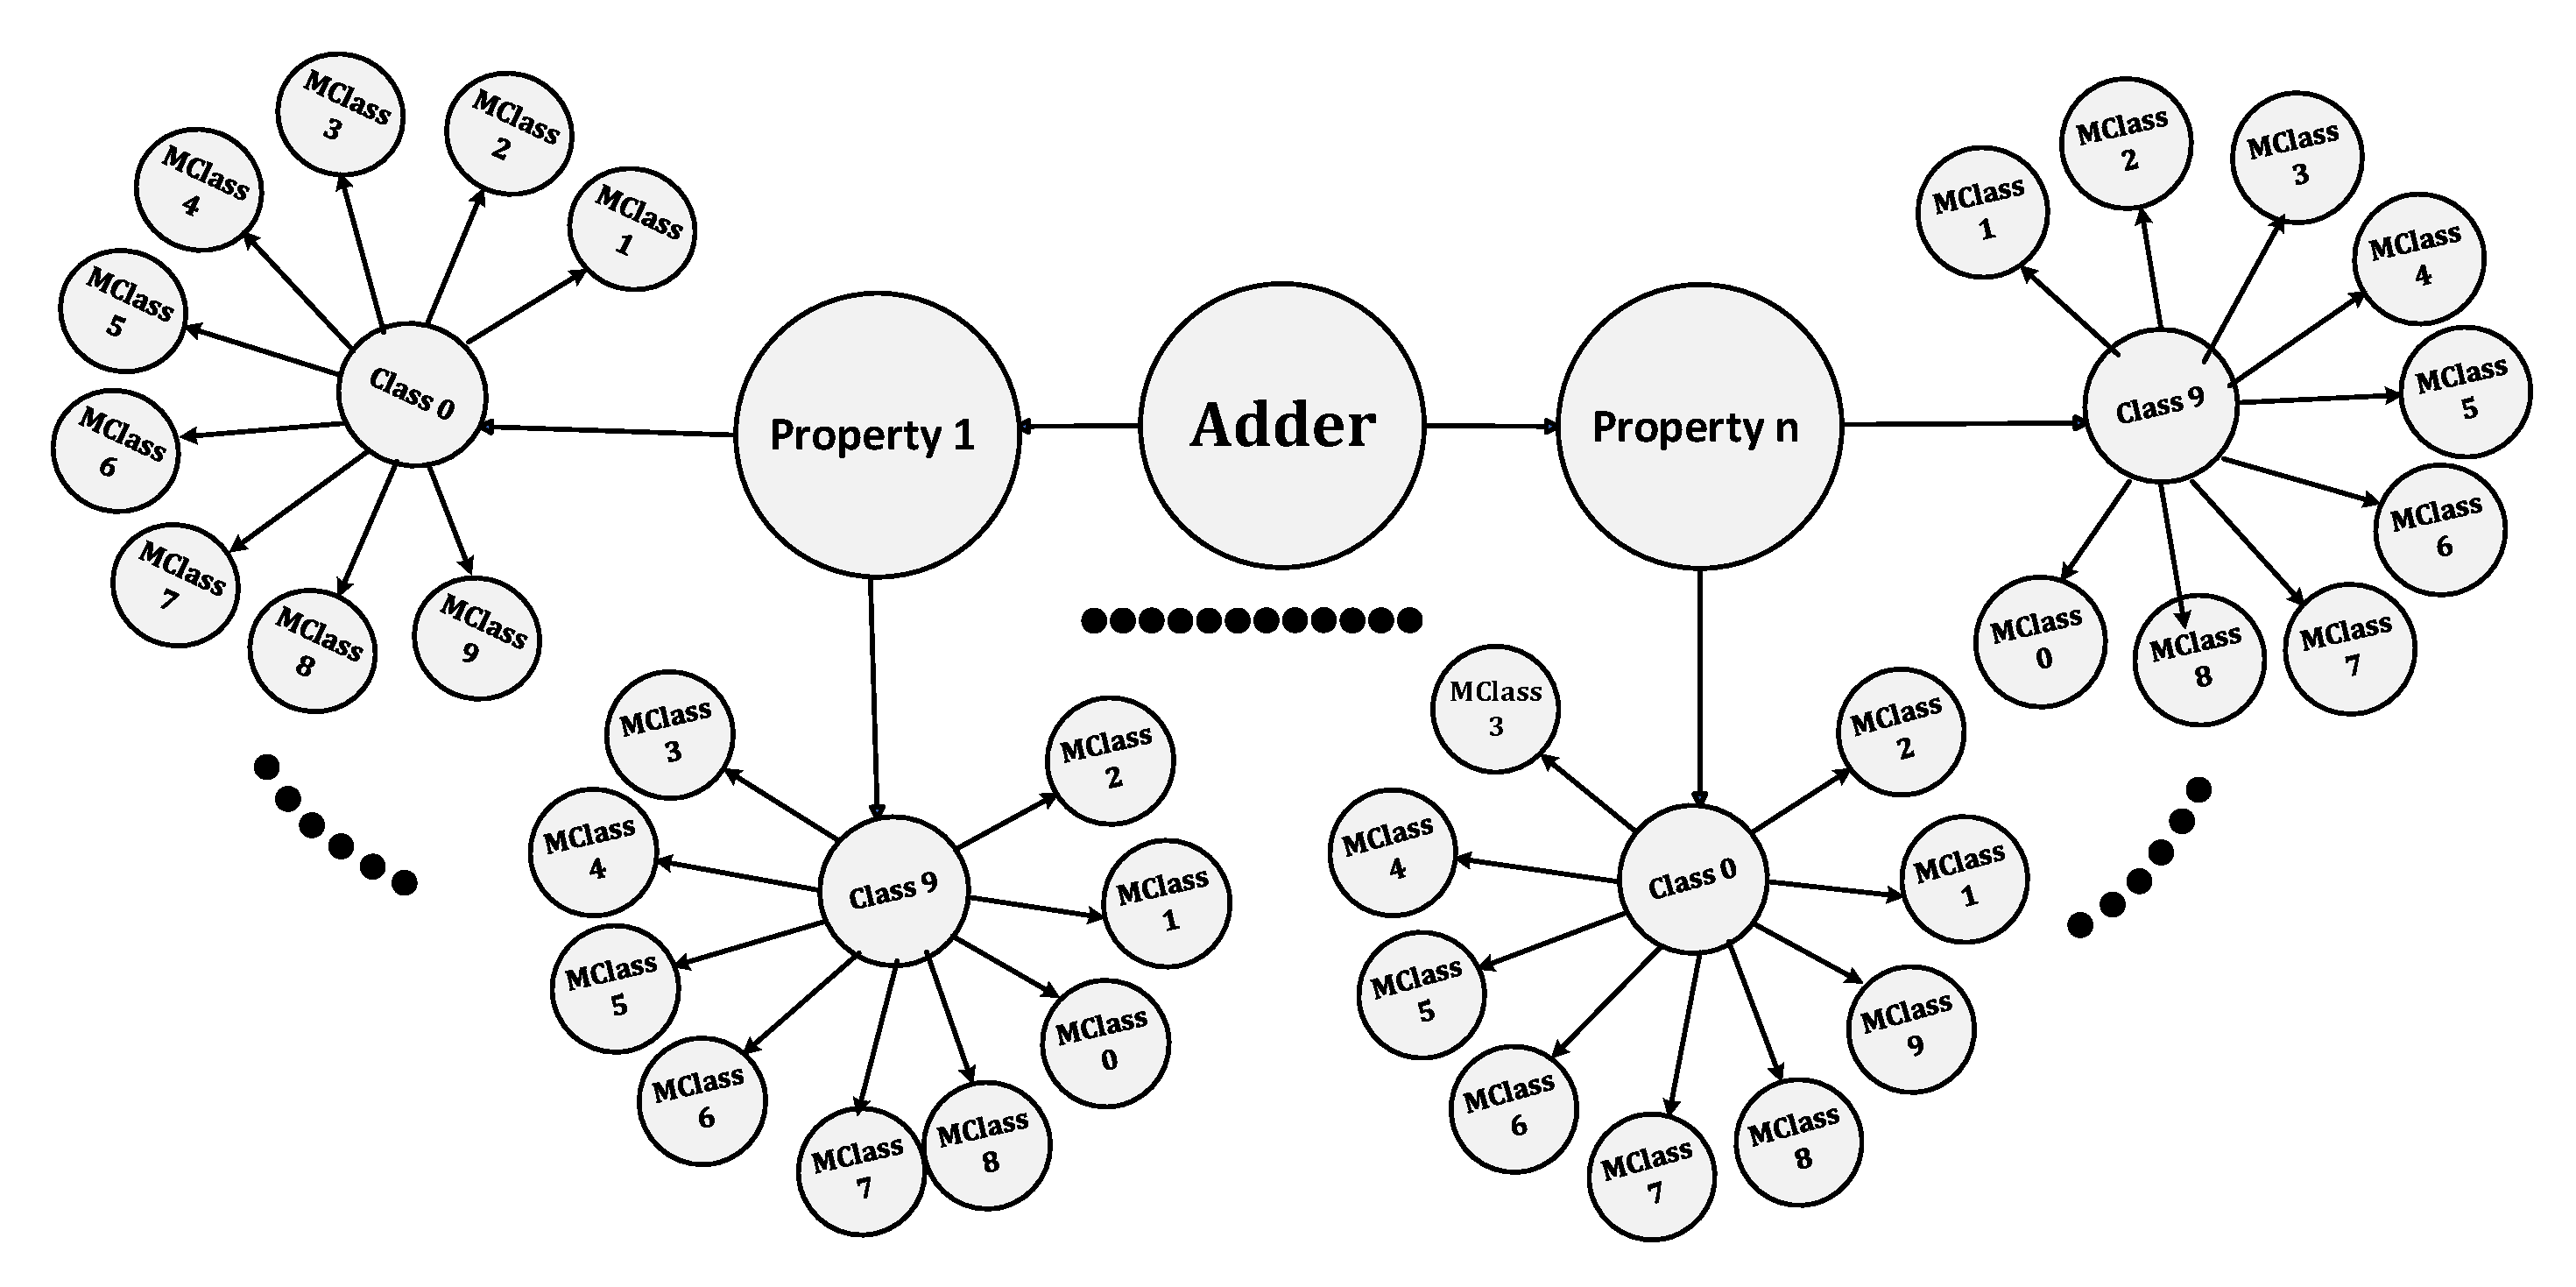
\includegraphics[width=1\textwidth]{figures/step5.pdf}
    \caption{Error Summarization}
    \label{Summarization}
\end{figure*}

\section{Gradient-Based Test Generation}

\begin{algorithm}
    \caption{Test Case Generation via Gradient-Based Attacks}
    \begin{tabular}{l l}
    \textbf{Input:} & Model $\mathcal{M}$ with bounds [0, 1], \\
    & Set of images $\mathcal{I} = \{i_1, i_2, \ldots, i_n\}$, \\
    & Corresponding labels $\mathcal{L} = \{l_1, l_2, \ldots, l_n\}$, \\
    & Perturbation magnitudes $\mathcal{E} = \{\epsilon_1, \epsilon_2, \ldots, \epsilon_k\}$, \\
    & Set of attacks $\mathcal{A} = \{A_1, A_2, \ldots, A_m\}$. \\
    \textbf{Output:} & Set of test cases $\bigcup TestCases_{ij}$. \\
    \textbf{Procedure:} & GenerateTestCases($\mathcal{M}$, $\mathcal{I}$, $\mathcal{L}$, $\mathcal{E}$, $\mathcal{A}$) \\
    & \quad \textbf{for} each attack $A_j$ in $\mathcal{A}$ \\
    & \quad \quad \textbf{for} each $\epsilon_i$ in $\mathcal{E}$ \\
    & \quad \quad \quad Generate testcases  $Adv_{ij} = A_j(\mathcal{M}, \mathcal{I}, \epsilon_i)$ \\
    & \quad \quad \quad Verify the $Adv_{ij}$ to obtain $V_{ij}$ \\
    & \quad \quad \quad Evaluate $V_{ij}$ against $\mathcal{L}$ to determine $isRobust_{ij}$ \\
    & \quad \quad \quad Compile test cases $TestCases_{ij} = \{Adv_{ij}, isRobust_{ij}\}$ \\
    & \quad \quad \textbf{end for} \\
    & \quad \textbf{end for} \\
    & \quad \textbf{return} $\bigcup TestCases_{ij}$ \\
    \end{tabular}
\end{algorithm}
